\documentclass[
	a4paper
]{scrartcl}

% PDF/A Compliance
\usepackage[a-2b]{pdfx}

% add unicode support and use german as language
\usepackage[utf8]{inputenc}
\usepackage[ngerman]{babel}

% Use Helvetica as font
\usepackage[scaled]{helvet}
\renewcommand\familydefault{\sfdefault}

% Better tables
\usepackage{tabularx}

% Better enumerisation env
\usepackage{enumitem}

% Use graphics
\usepackage{graphicx}

% Have subfigures and captions
\usepackage{subcaption}

% Be able to include PDFs in the file
\usepackage{pdfpages}

% Have custom abstract heading
\usepackage{abstract}

% Need a list of equation
\usepackage{tocloft}
\usepackage{ragged2e}

% Better equation environment
\usepackage{amsmath}

% Symbols for most SI units
\usepackage{siunitx}

\usepackage{csquotes}

% Clickable Links to Websites and sections
\usepackage{hyperref}

% Change page rotation
\usepackage{pdflscape}

% Symbols like checkmark
\usepackage{amssymb}
\usepackage{pifont}

\usepackage[absolute]{textpos}

% Change line spacing
\renewcommand{\baselinestretch}{0.9}

%%% PATH DEFINITIONS %%%
\graphicspath{{./img/}}

%%% DOCUMENT %%%

\begin{document}

\pagenumbering{gobble}

\begin{textblock*}{5cm}[0,0](15cm,0.7cm)
	
\includegraphics[keepaspectratio,width=5cm]{img/HSLU_Logo}
\end{textblock*}

\vspace*{2cm}

\noindent
\textbf{\LARGE{Suche von mit RFID-ausgerüsteten Einzelexemplaren in vollautomatischem
Behälter-Hochregallager}} \\

\vspace{0.5em}

\bgroup
% Remove padding of the table
\setlength\tabcolsep{0cm}

% Table itself
\begin{large}
\noindent
\begin{tabularx}{\textwidth}{p{5cm}X}
	\textbf{Themenbereiche:} & RFID, Automatisierte Arbeitsprozesse, Machbarkeitsstudie\\
	\textbf{Studierende:} & Pascal Baumann, Dane Wicki\\
	\textbf{Betreuungsperson:} & Martin Jud\\
	\textbf{Experte:} & Urs Gehrig\\
	\textbf{Auftraggebende:} & Verein Kooperative Speicherbibliothek Schweiz\\
	\textbf{Keywords:} & Logistik, RFID, Machbarkeitsstudie, Suchalgorithmus\\
\end{tabularx}
\end{large}
\egroup

\section{Aufgabenstellung}
In der Kooperativen Speicherbibliothek Schweiz werden Exemplare der dem Verein zugehörigen Bibliotheken eingelagert. Das heisst, das Exemplar der Bibliothek wird gereinigt und inventarisiert eingelagert. Sollte ein Bibliotheksbenutzer ein Exemplar dieses Werks anfordern, wird das Exemplar per Kurier an die jeweilige Bibliothek verschickt. Journale oder Magazine werden vorzugsweise eingescannt und in digitaler Form an den Benutzer übergeben, sofern dies so vom Benutzer bestellt wurde. Sowohl die beteiligten Bibliotheken, wie auch die Bibliotheksbenutzer sind daher an einer zeitgerechten Lieferung interessiert. Dies bedeutet für die Speicherbibliothek, dass alle Prozesse und Abläufe effizient und zuverlässig ablaufen müssen. Verzögerungen in Zwischenschritten können sich auf die ganze Auslieferung des Exemplars, in physischer oder digitaler Form, auswirken.

Ziel dieser Arbeit ist es, mittels einer Machbarkeitsstudie und einem Proof of Concept zu untersuchen, ob es technisch realisierbar ist, Exemplare, welche mit RFID Tags ausgerüstet sind, im Hochregallager der Speicherbibliothek zu finden.

Insbesondere sind dem Kunden folgende Resultate vorzulegen:
\begin{itemize}[noitemsep]
	\item Zwei ausgearbeiteten Konzepte
	\item Eine Machbarkeitsstudie zu einem ausgewählten Konzept
	\item Eine Dokumentation der Referenzimplementation der Machbarkeitsstudie
\end{itemize}

\vspace{0.5em}
\noindent
\begin{textblock*}{5cm}[0,0](14.93cm,277mm)
	
\includegraphics[keepaspectratio,width=5cm]{img/FHZ_Logo}
\end{textblock*}

\newpage

\begin{textblock*}{5cm}[0,0](15cm,0.7cm)
	
\includegraphics[keepaspectratio,width=2.7cm]{img/HSLU_Logo_Header}
\end{textblock*}

\section{Ergebnisse}
Wie in der Aufgabenstellung beschrieben, wurden zwei Konzepte ausgearbeitet. Während das Erste sich auf das automatische Auffinden von Exemplaren im Hochregallager konzentriert, befasst sich das zweite Konzept mit der Entwicklung einer Kontrollstation, welches deplatzierte Exemplare vor der Einlagerung identifizieren kann und den betreffenden Behälter aus dem Einlagerungsprozess ausschliesst (in Abbildung \ref{fig:PosAntennen} sind die Antennenpositionen dieser Station dargestellt).

\begin{figure}[htb]
	\centering
	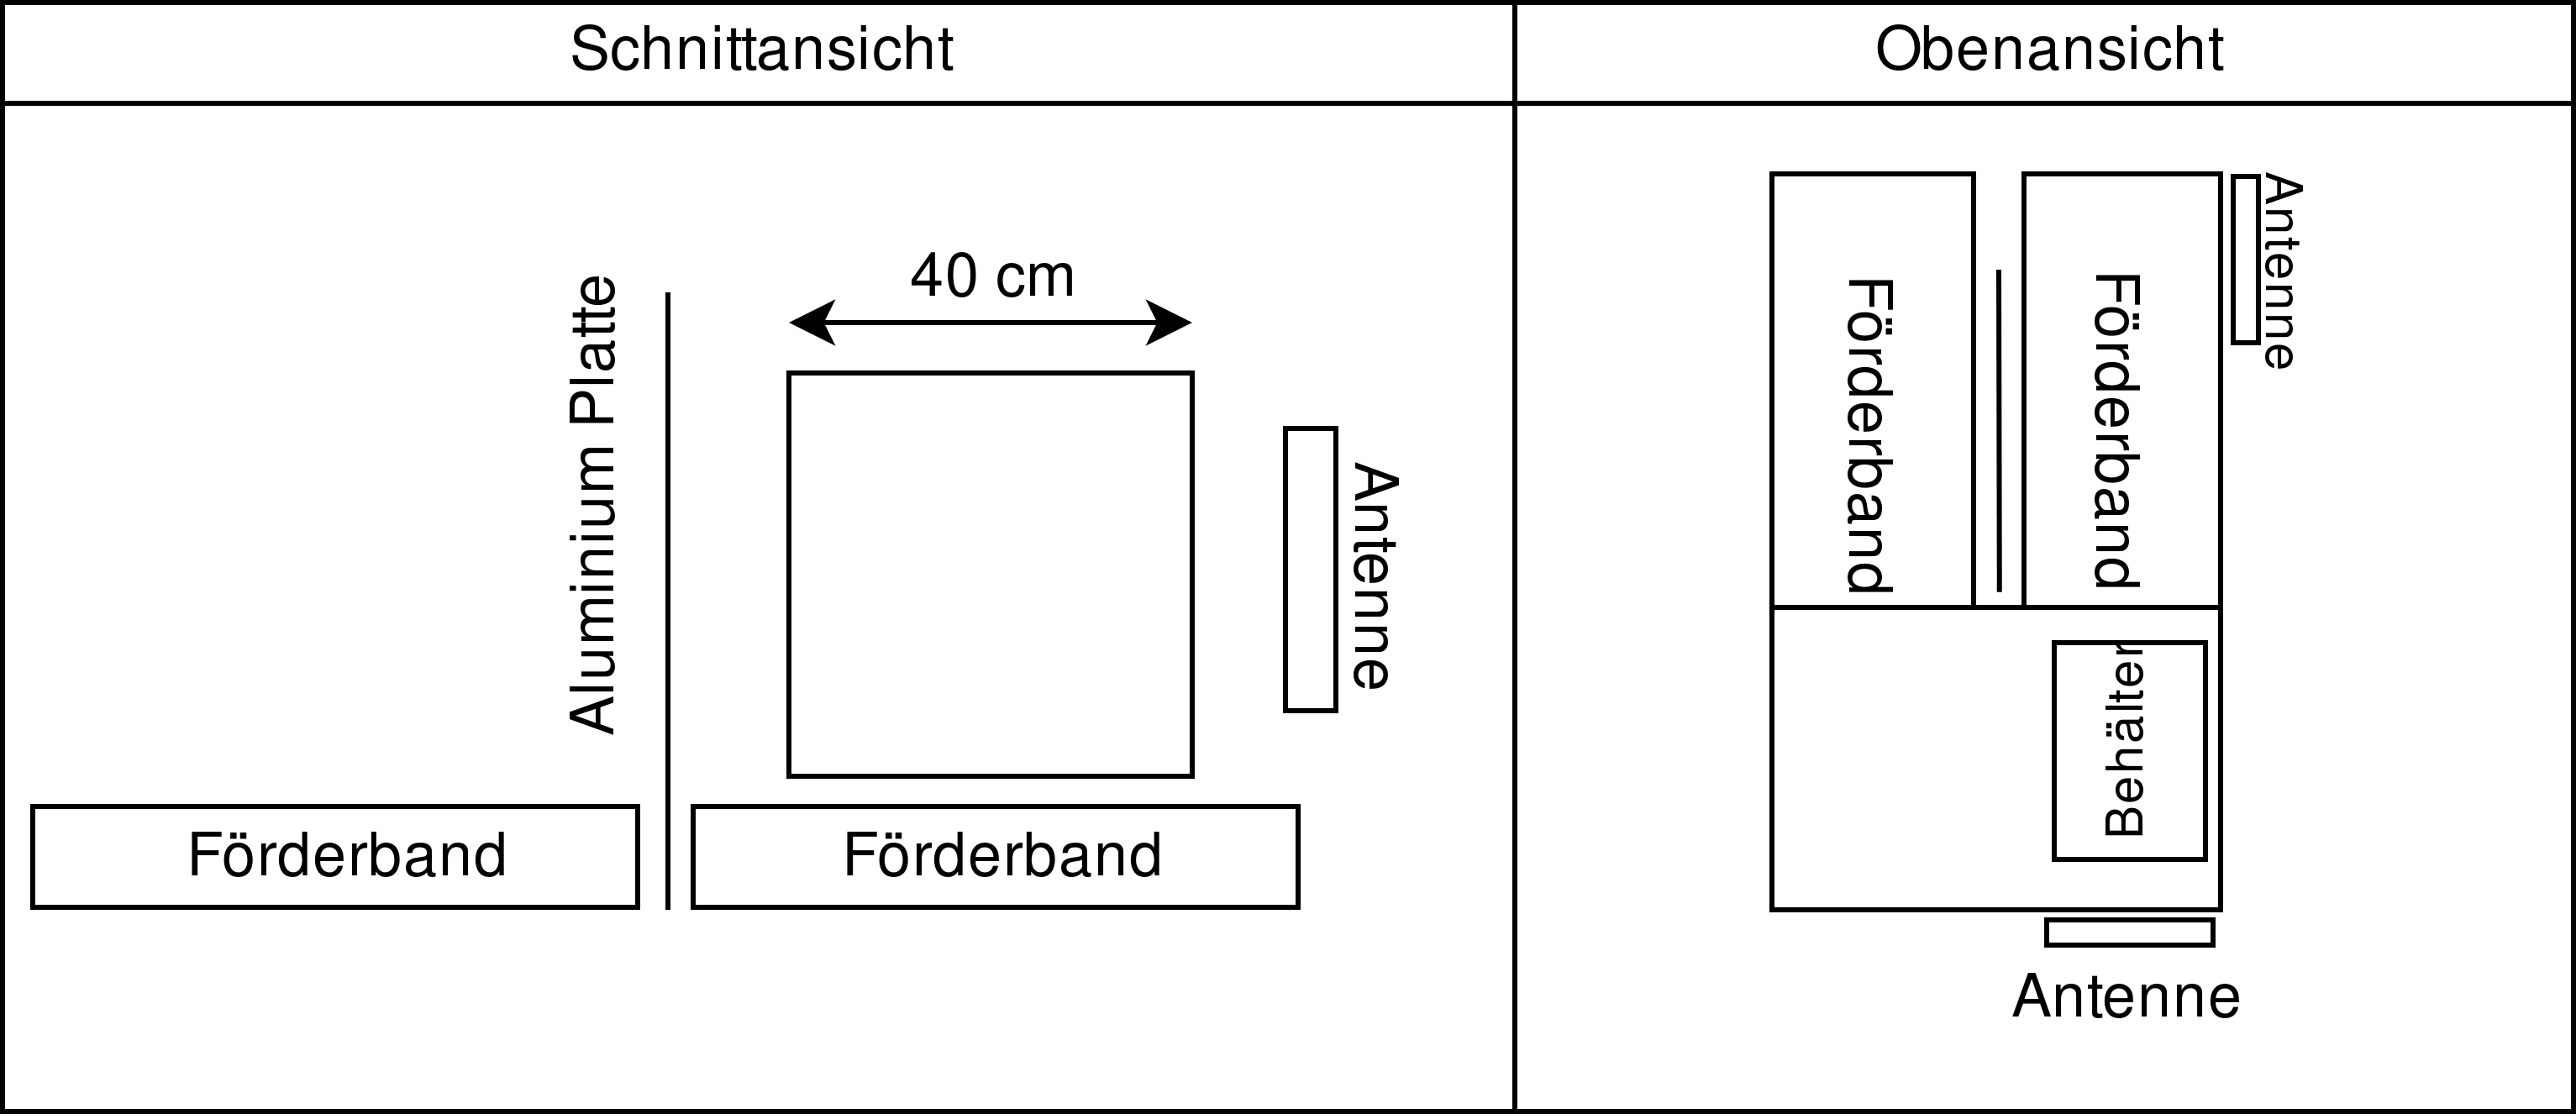
\includegraphics[keepaspectratio,width=\textwidth]{Positionierung_Antennen}
	\caption{Positionierung der LongRange Antennen des zweiten Konzepts}
	\label{fig:PosAntennen}
\end{figure}

In der darauffolgenden Versuchsphase konnte verifiziert werden, dass die Hardware, welche im Moment auf dem Markt existiert, für das Konzept der vollautomatischen Suche im Hochregallager, nicht geeignet ist und daher dieses für die Machbarkeitsstudie nicht weiter beachtet wurde.

Für die Machbarkeitsstudie wurde daher das Konzept der Kontrollstation ausgewählt. Die Machbarkeitsstudie kam zum Schluss, dass diese Lösung technisch machbar ist, und sich finanziell für den Kunden lohnt. Sie empfiehlt weiter die Implementierung des Konzeptes in einer weiteren Bachelorarbeit. Um die Ergebnisse der Machbarkeitsstudie zu validieren wurde eine Referenzimplementation erarbeitet, welche beim Kunden vor Ort das Lösungskonzept der Kontrollstation verifizierte.

\section{Lösungskonzept}
Das ganze Projekt wurde iterativ-inkrementell in zweiwöchigen Sprints durchgeführt. Da das Projekt jedoch mit sehr vielen Unbekannten konfrontiert war, entstand dabei nicht ein Prototyp, welcher durch das ganze Projekt weiterentwickelt wurde, sondern eine Anzahl unterschiedlicher Artefakte wie Anleitungen, Konzepte, Versuche, Machbarkeitsstudie, und eine Referenzimplementation.

\begin{textblock*}{5cm}[0,0](14.93cm,277mm)
	
\includegraphics[keepaspectratio,width=5cm]{img/FHZ_Logo}
\end{textblock*}

\newpage

\begin{textblock*}{5cm}[0,0](15cm,0.7cm)
	
\includegraphics[keepaspectratio,width=2.7cm]{img/HSLU_Logo_Header}
\end{textblock*}

Von den zwei erarbeiteten Konzepte, wurde nur eines für die Machbarkeitsstudie weiter beachtet. Dieses sieht zwei LongRange HF RFID Antennen und einen in einem Mikrocomputer integrierten Leser vor. Die zwei Antennen werden für eine grössere Abdeckung und Wahrscheinlichkeit einer vollständigen Auslesung aller RFID Tags benötigt. Sollte ein deplatziertes Exemplar gefunden werden, so soll der Behälter direkt ausgeschleust werden. Die Machbarkeitsstudie identifiziert die Kosten dieser Lösung auf circa 20'000 CHF (10'000 für Anpassungen des Lagersystems, 5'500 für Mitarbeiterschulungen).

\section{Spezielle Herausforderungen}
Die Herausforderungen in diesem Projekt lagen vor allem in der Wissensbeschaffung. Beide Teammitglieder waren nicht vertraut mit der Durchführung einer Machbarkeitsstudie und es musste daher zuerst eine Recherche durchgeführt werden, wie eine Machbarkeitsstudie durchgeführt werden soll.

Weiter war die Beschaffung eines Budgets, für die Anschaffung der Hardware, eine spezielle Hürde. Keiner der identifizierten Hersteller konnten Leihgaben zur Verfügung stellen. Sowohl die Hochschule wie auch der Kunde konnten keine grösseren Geldbeträge zur Verfügung stellen, sodass die Beschaffung, durch eine erneute Identifizierung von weiteren Herstellern welche Ihren Sitz im asiatischen Raum haben, verzögert wurde.

\section{Ausblick}
Die Machbarkeitsstudie sieht vor, dass die erarbeitete Lösung in einer weiteren Bachelorarbeit durchgeführt wird. Weiter wird ein klarer Budgetbetrag vorgesehen, welcher vom Kunden erbracht werden muss, bevor die Arbeit durchgeführt werden kann. Namentlich ist dies die Anschaffung der Hardware vom vorgesehenen Hersteller und der Auftrag für die Bereitstellung einer Schnittstelle zur automatisierten Ausschleusung durch den Entwickler des Lagerverwaltungssystems.

Wird die Lösung wie im Konzept ausgearbeitet entwickelt, so besitzt sie einen grossen Neuheitsgrad, da HF RFID Chips in einer spezialisierten Umgebung (ausschliesslich Bibliotheken und deren Lager) eingesetzt werden. In diesem Umfeld existieren noch keine Fertiglösungen für ein System, welche diese Dichte von Tags verarbeiten kann.

\vspace{0.5em}
\noindent
\begin{textblock*}{5cm}[0,0](14.93cm,277mm)
	
\includegraphics[keepaspectratio,width=5cm]{img/FHZ_Logo}
\end{textblock*}
\end{document}
